% Chapter Template

\chapter{Ensayos y Resultados} % Main chapter title

\label{Chapter4} % Change X to a consecutive number; for referencing this chapter elsewhere, use \ref{ChapterX}

En este capítulo se describe la estrategia general de \textit{testing} del proyecto y se documentan los ensayos realizados en tres niveles de abstracción: a nivel de función, a nivel de módulo y a nivel de sistema.

%----------------------------------------------------------------------------------------
%	SECTION 1
%----------------------------------------------------------------------------------------

\section{Test Master Plan}
\label{sec:masterPlan}

Para la elaboración de un \textit{Test Master Plan} se tomaron elementos del paradigma de desarrollo basado el pruebas o TDD (por sus siglas en inglés, \textit{Test Driven Development}) como fue mencionado en en capítulo \ref{Chapter2}, subsección \ref{subsec:tdd}. 

Cabe destacar en este sentido, que en la planificación de las tareas del proyecto, primero se definieron los casos de prueba; luego se prepararon las herramientas de \textit{testing}; luego se implementaron los módulos y finalmente, se realizaron las pruebas. Esto puede observarse en el diagrama de \textit{Activity on Node} de la figura \ref{fig:AoN} en la sección \ref{sec:plan}.

Resultó necesario tener bien definidos los requisitos funcionales y sus criterios de aceptación.  Se debieron contemplar todos los casos posibles de uso, tanto exitosos como de error, con lo que se elaboró un documento \citep{TestMasterPlan} de casos de prueba por módulo  y de esta manera, se dio cumplimiento al requerimiento 1.2 indicado en la sección \ref{sec:requerimientos}.  

Se ensayó el código en tres niveles distintos de abstracción: a nivel de función, de módulo y de sistema, según se documenta en las subsecciones \ref{subsec:unitarias}, \ref{subsec:pruebasFuncionales} y \ref{subsec:pruebasSistema}, respectivamente. 

Asimismo, las pruebas sobre los módulos fueron diseñadas para evaluar únicamente la lógica principal de funcionamiento.  En cada caso, se debió abstraer al módulo bajo ensayo de otras capas o servicios que pudieran interactuar con su lógica principal, para lo cual se simuló el resultado de dichas interacciones con \textit{mocks}. 


\subsection{Pruebas unitarias}
\label{subsec:unitarias}

Para realizar pruebas unitarias al código se utilizó el framework Ceedling \citep{ceedling} que se distribuye como una gema del lenguaje de programación ruby.  \textit{Ceedling} integra tres herramientas, \textit{Unity}, \textit{Cmock} y \textit{CException} y se encarga de compilar y ejecutar los test sobre el código.

A continuación se presentan los casos de prueba que se definieron para ensayar con test unitarios, las funciones de los cuatro módulos desarrollados.  

Se utilizó una técnica para expandir la cantidad de test posibles que consiste desdoblar los test sobre cada caracterísitca a evaluar en un test positivo, un test negativo y otro de rango cuando esto último fuera pertinente.  Esto significa evaluar cuando una condición se cumple (positivo) y tambien cómo reaccioná el sistema cuando no se cumple (negativo).  Los test de rango permiten evaluar si los parámetros y resultados que devuelven las funciones ensayadas se encuentran dentro de los valores previsto.

\subsubsection{Módulo Almacenamiento}

En la figura \ref{fig:test_almacenamiento} se recopilan los casos de prueba para el módulo de almacenamiento.  En la primer columna se incluye un código de indentificación único del test que permite realizar la trazabilidad con los requerimientos.

\begin{figure}[htpb]
	\centering
	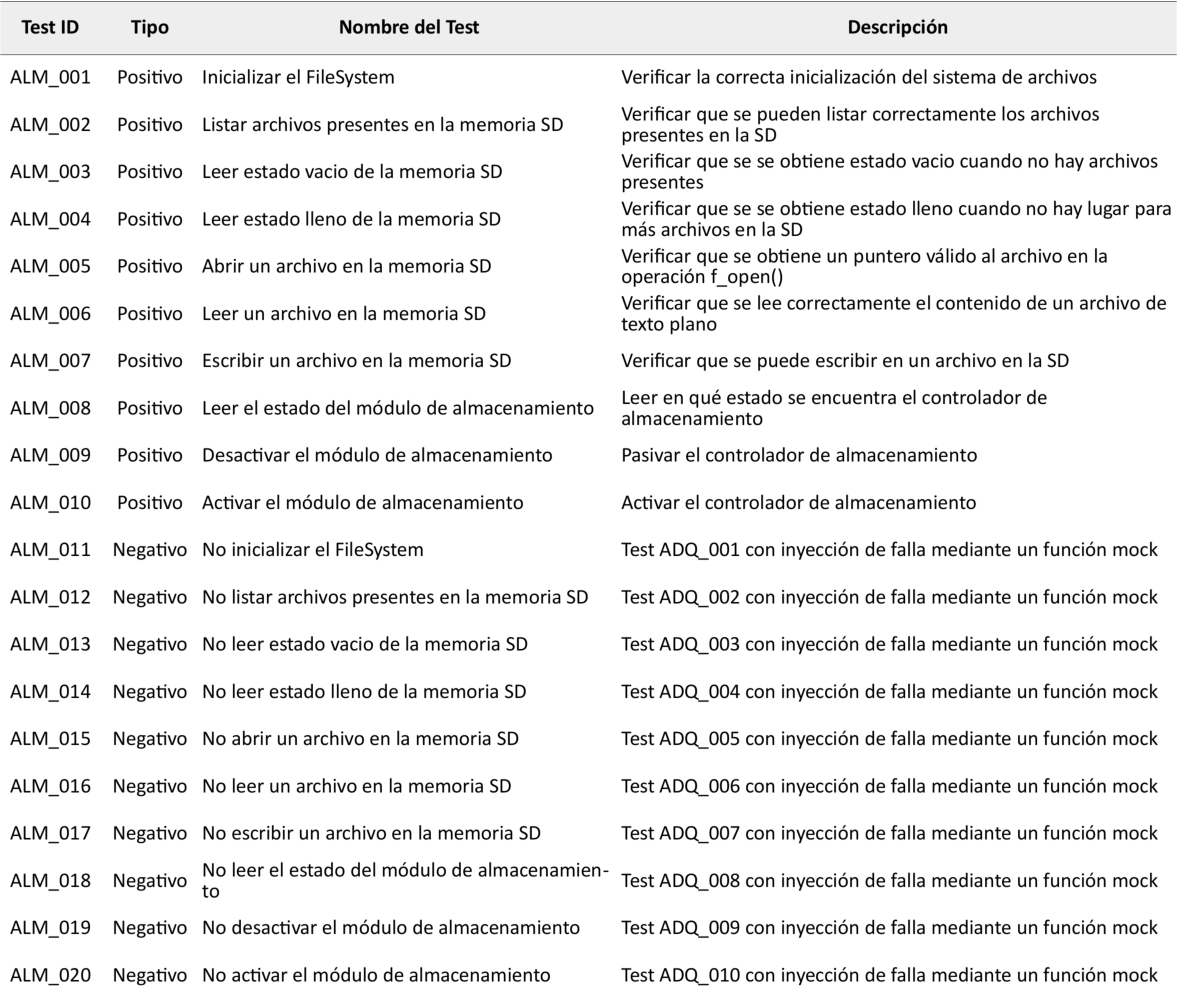
\includegraphics[width=\textwidth]{./Figures/TestSD.pdf}
	\caption{Casos de prueba para test unitarios del módulo de almacenamiento}
	\label{fig:test_almacenamiento}
\end{figure}

Los test negativos se resolvieron con funciones mock que simulan el comportamientos erroneo del componente bajo prueba.  No se realizaron test de rango para este módulo.

Todos los test ejecutados resultaron exitosos.

\subsubsection{Módulo adquisición}

Los casos de prueba para el módulo de adquisición se presentan en la figura \ref{fig:test_adquisición}. Para este módulo se definieron diez test de rango además de los test positivos y negativos.  Para éstos últimos se utilizaron funciones \textit{mock} para simular una falla.

\begin{figure}[!htpb]
	\centering
	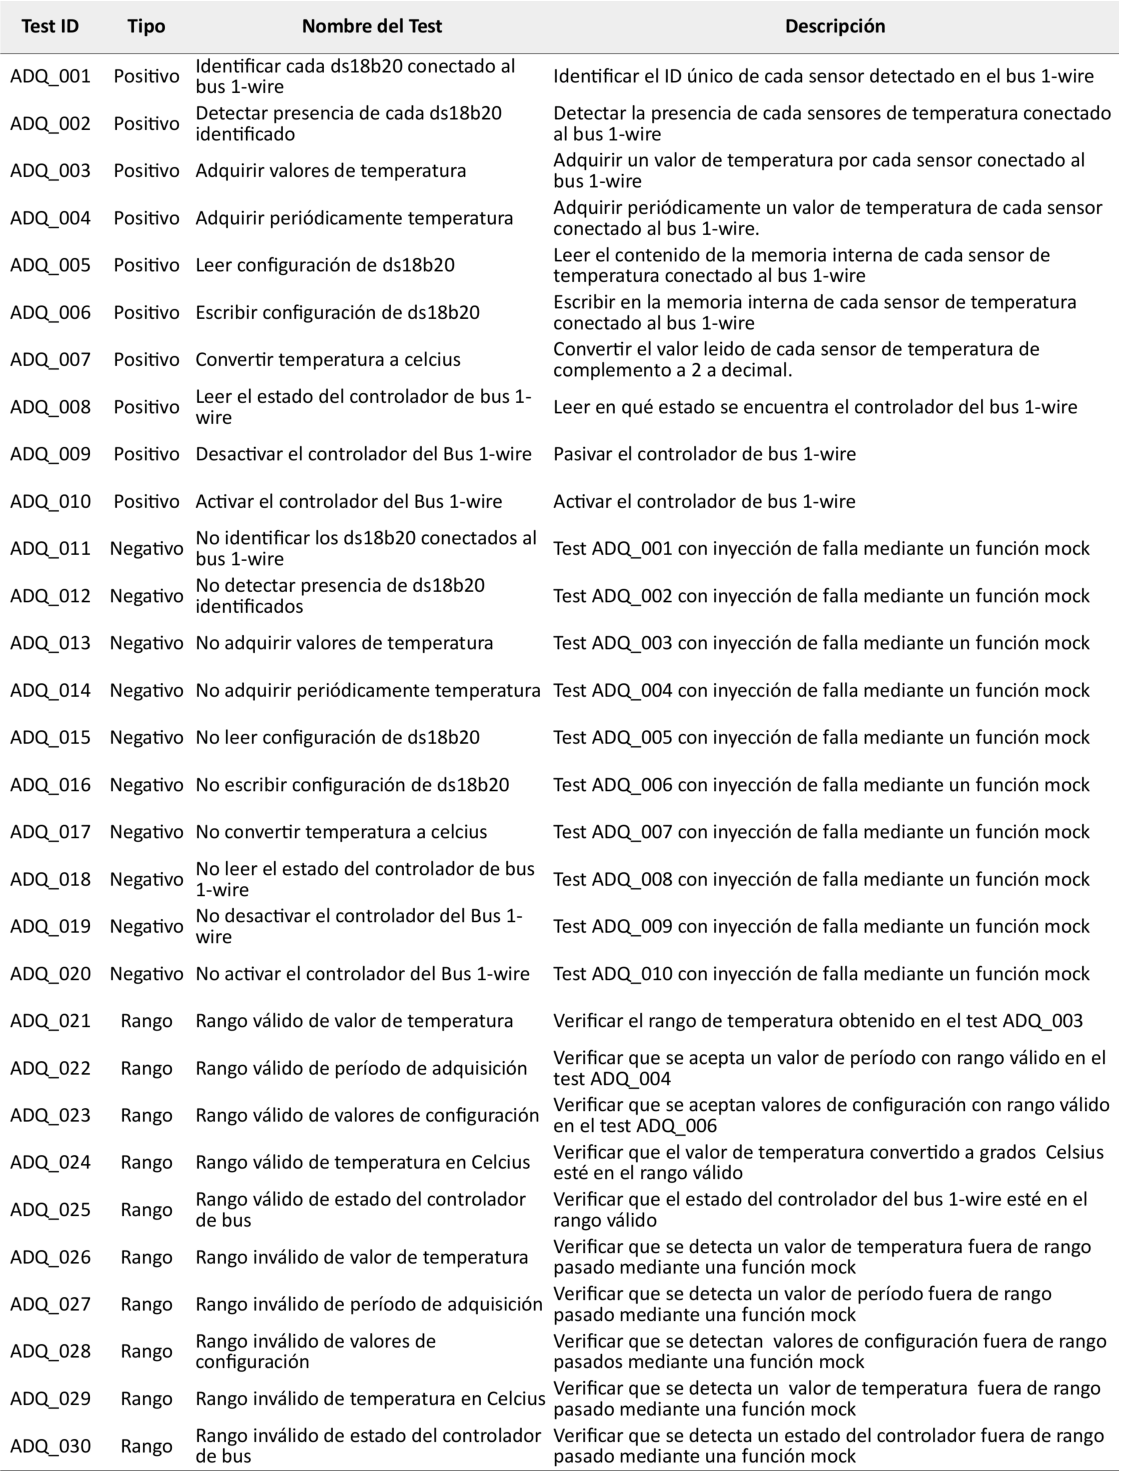
\includegraphics[width=\textwidth]{./Figures/TestADQ.pdf}
	\caption{Casos de prueba para test unitarios del módulo de adquisición}
	\label{fig:test_adquisición}
\end{figure}

Todos los test ejecutados resultaron exitosos.

\subsubsection{Módulo HMI}

\subsubsection{Módulo Control}

\subsection{Pruebas funcionales}
\label{subsec:pruebasFuncionales}


[\textbf{pruebas sobre las MEF de cada bloque}]

\subsection{Pruebas de sistema}
\label{subsec:pruebasSistema}

[\textbf{Pruebas}]